\documentclass[a4paper,12pt]{article}
\usepackage{../../mypackages}
\usepackage{../../macros}

\setlength{\parindent}{0pt}


\begin{document}

\title{Chapitre 2 : Les ions}
\author{N. Bancel}
\date{Octobre 2024}
\maketitle

\section{Connaissances à connaître pour le contrôle}

\begin{tcolorbox}[colback=blue!10, colframe=blue!80, title=]
  \begin{itemize}
    \item Numéro atomique de l'atome
    \item Définition d'un ion (et la différence entre un cation et un anion)
    \item Les méthodes d'identification des ions
    \item Différence entre électriquement neutre et conducteur
  \end{itemize}
\end{tcolorbox}

\section{Rappels : constitution d'un atome}



La matière est constituée de petits « grains » de matière appelés \textbf{atomes}. Le diamètre d’un atome est de l’ordre de $10^{-10} \, m = 0.1 \, nm$.

\begin{tcolorbox}[colback=blue!10, colframe=blue!80, title=]
\textbf{Un atome est constitué d’un noyau central autour duquel gravitent un ou plusieurs électrons.}
\end{tcolorbox}

Le noyau et les électrons sont séparés par du \textbf{vide}. Il existe une centaine d’atomes différents. Leurs noms, symboles et caractéristiques sont répertoriés dans le \textbf{tableau périodique des éléments}.

\begin{tcolorbox}[colback=purple!10, colframe=purple!80, title=]
\textbf{Le noyau est chargé positivement} \par 
\textbf{Le numéro atomique Z indique le nombre de charges positives du noyau.} \par
\textbf{Un atome est électriquement neutre.}
\end{tcolorbox}


La charge positive du noyau est compensée par les charges négatives, portées chacune par un électron.

\begin{figure}[H]
  \centering
  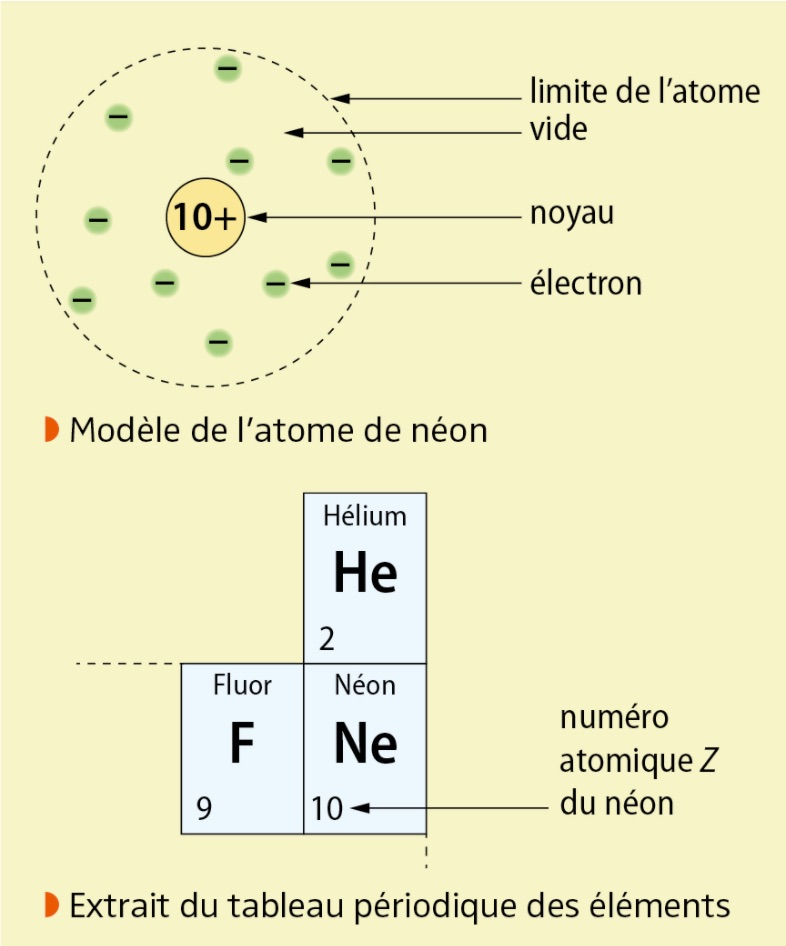
\includegraphics[width=0.8\linewidth]{img1.jpg}
  \caption{\label{} L'atome}
\end{figure}

\section*{Les ions}

\begin{tcolorbox}[colback=green!10, colframe=green!80, title=Définition]
\textbf{Un ion est un atome (ou un groupe d’atomes) qui a perdu ou gagné un ou plusieurs électrons. Il est électriquement chargé.} \\
Si des électrons sont perdus, l’ion formé est \textbf{positif} : c’est un \textbf{cation}. Si des électrons sont gagnés, l’ion formé est \textbf{négatif} : c’est un \textbf{anion}.
\end{tcolorbox}

\subsection*{Formule chimique}

La formule chimique d’un ion se compose du symbole chimique de l’atome (ou du groupe d’atomes) initial suivi de la charge de l’ion, inscrite en exposant.

\subsection*{Conséquences pour une solution}

Comme un ion est électriquement chargé, la présence d’ions rend une solution conductrice.

\begin{figure}[H]
  \centering
  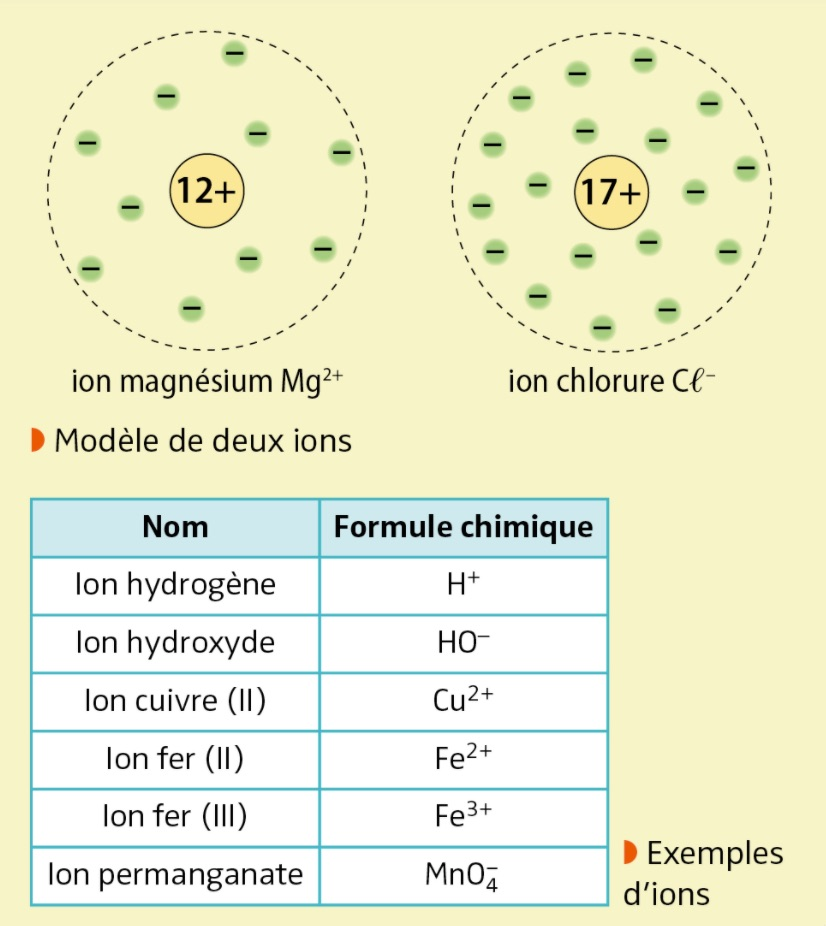
\includegraphics[width=0.9\linewidth]{img2.jpg}
  \caption{\label{} Les ions}
\end{figure}

\section*{Identification d'ions dans une solution}

\subsection*{Première approche}

Une solution étant électriquement neutre, si elle contient des cations, elle contient nécessairement des anions aussi.

\begin{tcolorbox}[colback=purple!10, colframe=purple!80]
\textbf{Le nom donné à une solution renseigne sur sa composition.}
\end{tcolorbox}

Par exemple, une solution de chlorure de sodium contient des ions chlorure Cl\textsuperscript{-} et des ions sodium Na\textsuperscript{+}. Il est sous-entendu que le solvant est ici l'eau.

\begin{figure}[H]
  \centering
  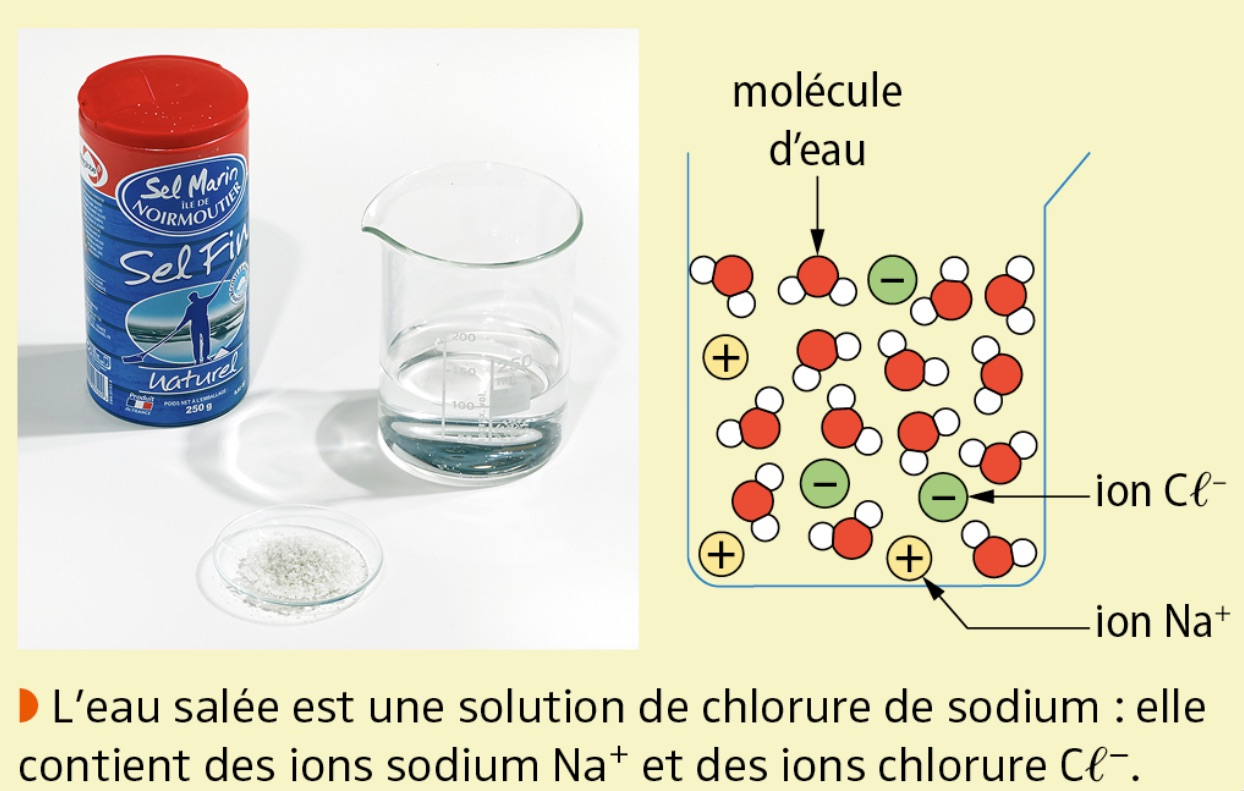
\includegraphics[width=0.9\linewidth]{img4.jpg}
  \caption{\label{} Les ions}
\end{figure}

\subsection*{Identification d'ions}

\begin{tcolorbox}[colback=purple!10, colframe=purple!80]
\textbf{Il est possible d'identifier certains ions présents dans une solution grâce à des tests caractéristiques.} \\
Au contact d'un réactif adapté, chaque ion forme un précipité caractéristique.
\end{tcolorbox}

Ces tests se réalisent sur un \textbf{échantillon} de la solution et jamais sur la totalité de la solution.

\begin{figure}[H]
  \centering
  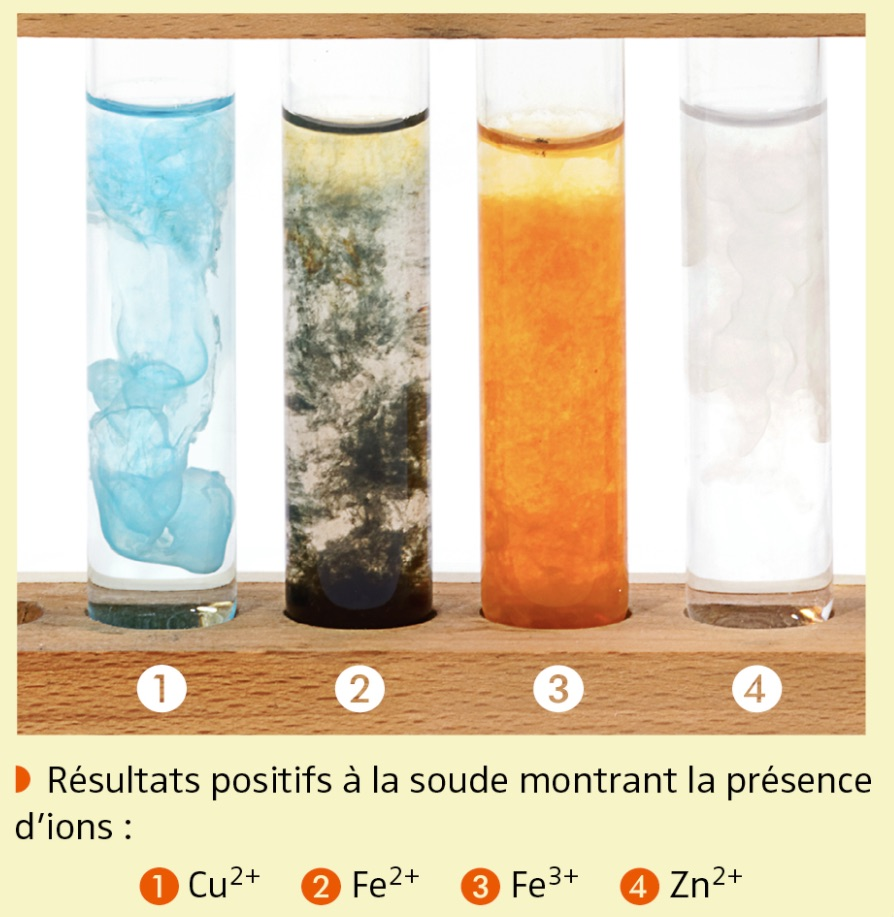
\includegraphics[width=0.9\linewidth]{img3.jpg}
  \caption{\label{} Les ions}
\end{figure}

\section*{L'électroneutralité en solution aqueuse}

\begin{align*}
  \ce{NaCl &->[\text{en solution}] Na^+ + Cl^-} \\
  \ce{KCl &->[\text{en solution}] K^+ + Cl^-} \\
  \ce{NaOH &->[\text{en solution}] Na^+ + OH^-} \\
  \ce{Na2SO4 &->[\text{en solution}] 2Na^+ + SO4^{2-}} \quad \text{(cette solution contient 2 fois plus d’ions \ce{Na^+} que d’ions \ce{SO4^{2-}})} \\
  \ce{Al2(SO4)3 &->[\text{en solution}] 2Al^{3+} + 3SO4^{2-}} \\
  \ce{Fe2(SO4)3 &->[\text{en solution}] 2Fe^{3+} + 3SO4^{2-}} \\
  \ce{AlCl3 &->[\text{en solution}] Al^{3+} + 3Cl^-} \\
  \ce{CuSO4 &->[\text{en solution}] Cu^{2+} + SO4^{2-}}
\end{align*}

\end{document}







